面向对象编程(OOP)为我们提供了一种思考方式,可以用类及关系来描述现实世界。函数式编程是一种完全不同的编程范式,它允许我们专注于函数结构,而不是代码的物理结构。学习和使用函数式编程很有用。首先,它是一种新的范式,可使你以非常不同的方式思考。解决问题需要灵活的思维,执着于单一范式的人往往会为任何问题提供类似的解决方案,而最优雅的解决方案需要更好的方法。掌握函数式编程为开发人员提供了一种新技能,可以帮助他们提供更好的问题解决方案。其次,使用函数式编程减少了软件中的错误数量。函数式编程采用独特方法的最大原因之一是:将程序分解为函数,每个函数都不修改数据的状态。\par
本章中,我们将讨论函数式编程的基本模块以及范围。C++20中引入的range为我们提供了一种方法来组合算法,这样就可以处理数据集合。组合算法以便我们可以将它们按顺序应用到数据集合中,这是函数式编程的核心。 \par
本章中,我们将了解以下内容: \par

\begin{itemize}
	\item 函数式编程简介
	\item ranges库的介绍
	\item 纯函数
	\item 高阶函数
	\item 深入地研究递归
	\item C++中(函数式)的元编程
\end{itemize}

\noindent\textbf{}\ \par
\textbf{编译器要求} \ \par
g++编译器需要添加编译选项 \texttt{-std=c++2a} 来编译本章的代码。可以从这里获取本章的源码文件:https:/​/github.​com/PacktPublishing/Expert-CPP \par

\noindent\textbf{}\ \par
\textbf{函数式编程} \ \par
正如我们前面提到的,函数式编程是一种编程范式。构建程序时,可以将范式视为一种思考方式。C++是一种多范式语言,可以使用它在过程范式中开发程序,即一个接一个地执行语句。第3章中,我们讨论了面向对象方法,涉及到将一个复杂的系统分解为相互通信的对象。另一方面,函数式编程鼓励我们将系统分解为函数,而不是对象。表达式受一些输入,并一个产生输出,输出这可以用作另一个函数的输入。乍一看,似乎很简单,但是函数式编程包含了一些最初感觉很难掌握的规则和实践。然而,当你做到这一点时,大脑就会开启一种新的思维方式——功能性思维方式。 \par 
为了更清楚地说明这一点,让我们会从一个示例开始,这个示例将演示函数式编程的原理。假设得到了一个整数列表,需要计算其中的偶数个数。唯一的问题是我们应该分别计算所有向量中的偶数,并生成一个新向量,其中包含每个输入向量的计算结果。 \par
输入是一个矩阵,即向量中的向量。在C++中,最简单的表达方式是使用以下类型: \par

\begin{lstlisting}[caption={}]
std::vector<std::vector<int>>
\end{lstlisting}

我们可以通过使用类型别名来进一步简化前面的代码,如下所示: \par

\begin{lstlisting}[caption={}]
using IntMatrix = std::vector<std::vector<int>>;
\end{lstlisting}

下面是对这个问题的说明。我们有一串包含整数的向量,因此应该得到一个包含偶数计数的vector: \par

\begin{center}
	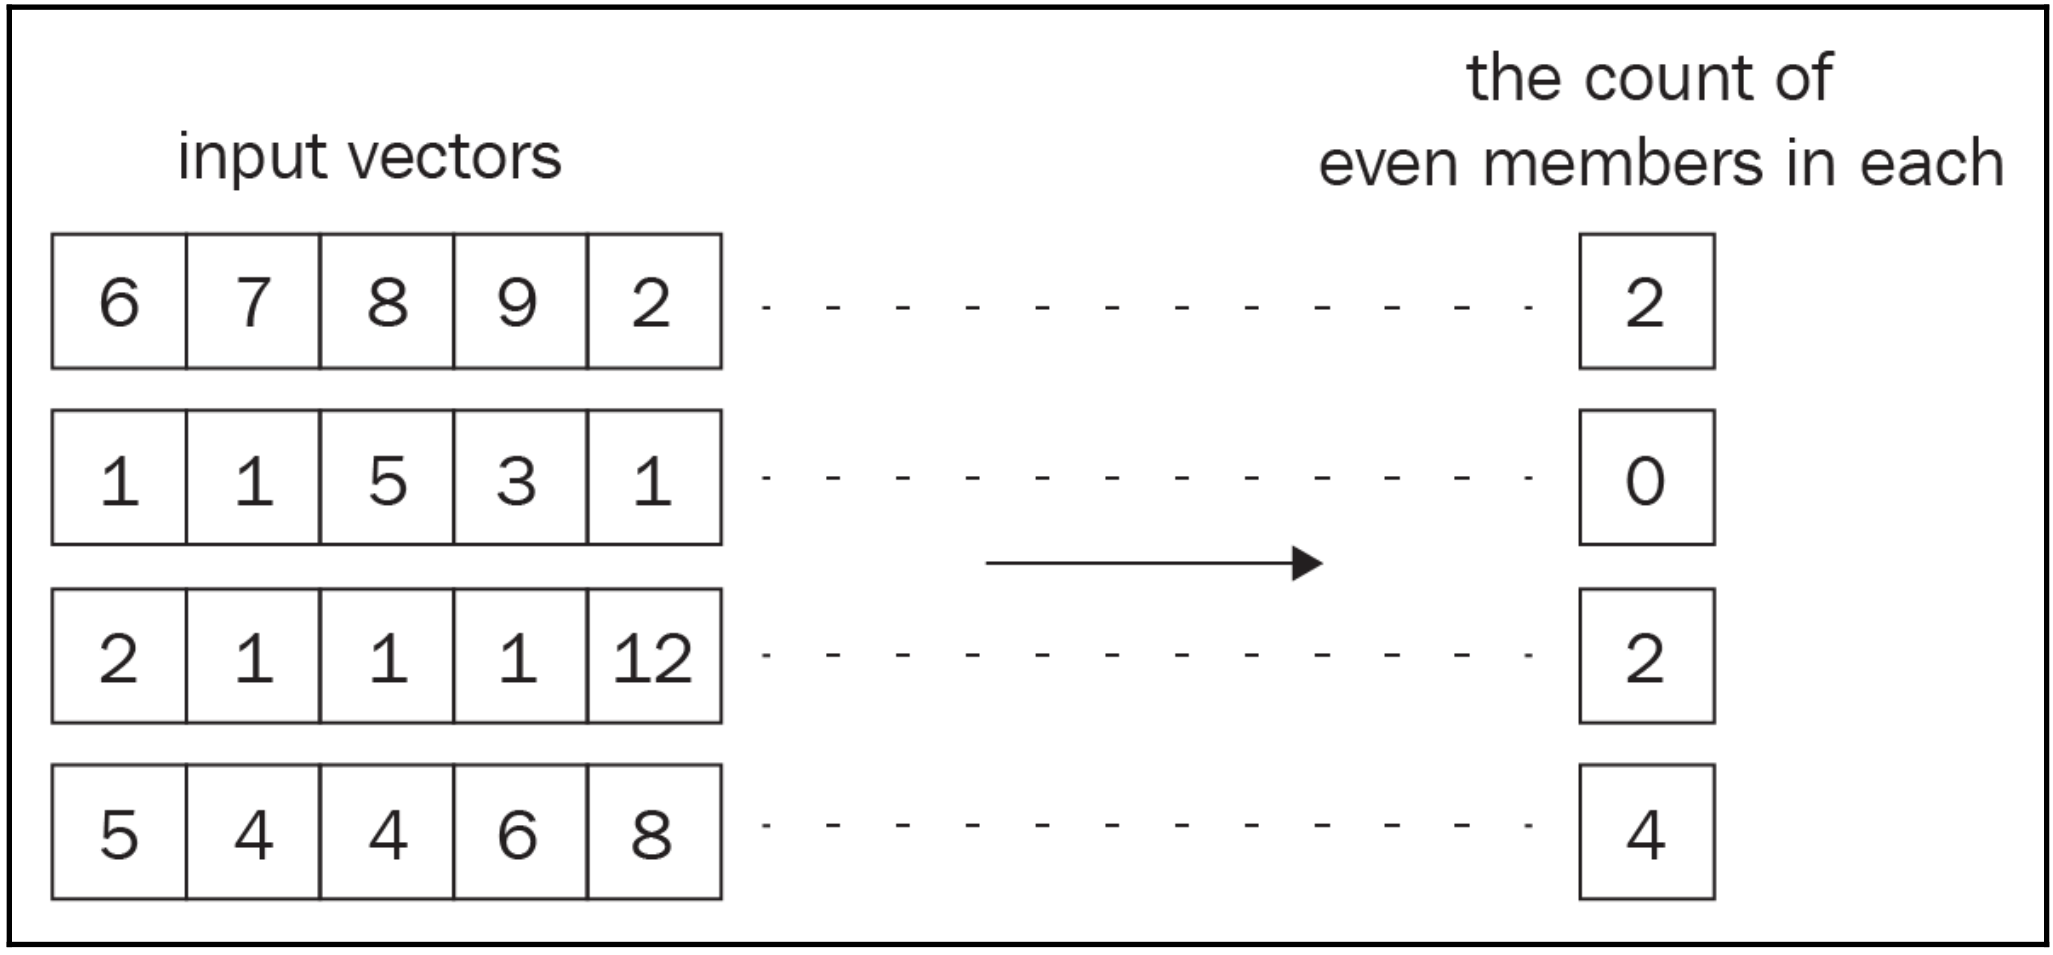
\includegraphics[width=0.6\textwidth]{content/Section-2/Chapter-7/1}
\end{center}

看看下面的函数。它以一个由整数向量组成的vector(也称为矩阵)作为它的参数。该函数计算偶数的数目: \par

\begin{lstlisting}[caption={}]
std::vector<int> count_all_evens(const IntMatrix& numbers)
{
	std::vector<int> even_numbers_count;
	for (const auto& number_line: numbers) {
		int even{0};
		for (const auto& number: number_line) {
			if (number % 2 == 0) {
				++even;
			}
		}
		even_numbers_count.push_back(even);
	}
	return even_numbers_count;
}
\end{lstlisting}

前面的函数保留一个vector来存储每个向量的偶数计数,输入为二维vector。对于检索到的每个vector,都将对其进行循环,并在每次遇到vector中的偶数时在计数器上增加1。完成每个向量的循环后,最终结果推入包含数字列表的vector中。我们现在继续,并将其分解为更小的函数。首先,我们将负责计算偶数的代码部分移动到单独的函数中。 \par
我们把它命名为count\underline{ }evens,如下所示: \par

\begin{lstlisting}[caption={}]
int count_evens(const std::vector<int>& number_line) {
	return std::count_if(number_line.begin(),
	number_line.end(), [](int num){return num % 2 == 0;});
}
\end{lstlisting}

注意如何使用count\underline{ }if()算法。它接受两个迭代器,并将它们分别放在容器的开头和结尾。它还接受第三个参数,一元谓词,集合的每个元素都会调用该谓词。我们传递一个lambda作为一元谓词,也可以使用任何其他可调用实体,例如函数指针、std::function等。 \par
现在有了独立的计数函数,我们可以在count\underline{ }all\underline{ }even()函数中调用它。下面是count\underline{ }all\underline{ }evens()在C++中函数式编程的实现: \par

\begin{lstlisting}[caption={}]
std::vector<int> count_all_evens(const std::vector<std::vector<int>>&
numbers) {
	return numbers | std::ranges::views::transform(count_evens);
}
\end{lstlisting}

深入研究前面的代码之前,我们需要达成一致意见——这里并不是|操作符的什么怪异用法,而是为了简化代码。将其与我们在本节开始时介绍的代码版本进行比较,两者的作用一样,但第二种——功能更简洁。另外,注意这个函数不保留或改变任何状态。这在函数式编程中至关重要,因为函数必须是纯函数。它接受一个参数,然后在不修改它的情况下处理它,并返回一个新值(通常基于输入)。函数式编程的第一个挑战是将一个任务分解为更小的、易于组合的独立函数。  \par
尽管是从命令式解决方案开始使用函数式解决方案,但在利用函数式编程范式时,这不是使用它的正确方式。应该改变思考问题的方式和处理问题的方式,而不是首先编写命令式代码,并修改它以获得函数式版本。读者应该经历从功能上思考的过程。所有的偶数的问题,我们使用一个vector解决问题。如果能找到解决单个vector问题的方法,就能解决所有vector问题。count\underline{ }evens()函数接受一个vector并产生单个值,如下图所示: \par

\begin{center}
	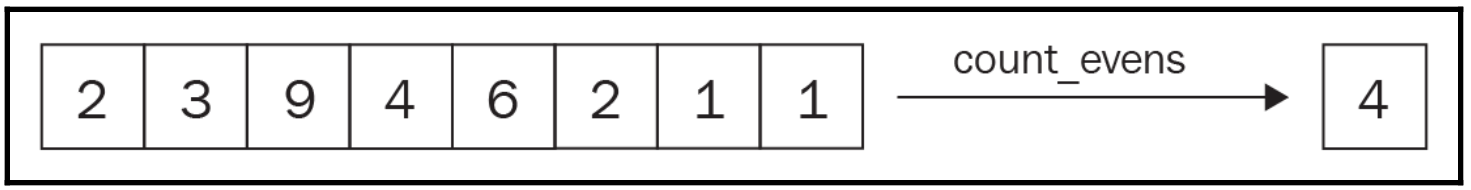
\includegraphics[width=0.6\textwidth]{content/Section-2/Chapter-7/2}
\end{center}

解决了vector的问题之后,我们应该通过将解应用到所有的向量,来继续解决最初的问题。transform()函数本质上完成了我们所需要的工作:它接受一个可以应用于单个值的函数,并对其进行转换,以处理一个集合。下面的图像说明了如何使用它来实现一个函数(count\underline{ }all\underline{ }evens),该函数可以处理来自一次只处理一个项的函数(count\underline{ }evens)的项的集合: \par

\begin{center}
	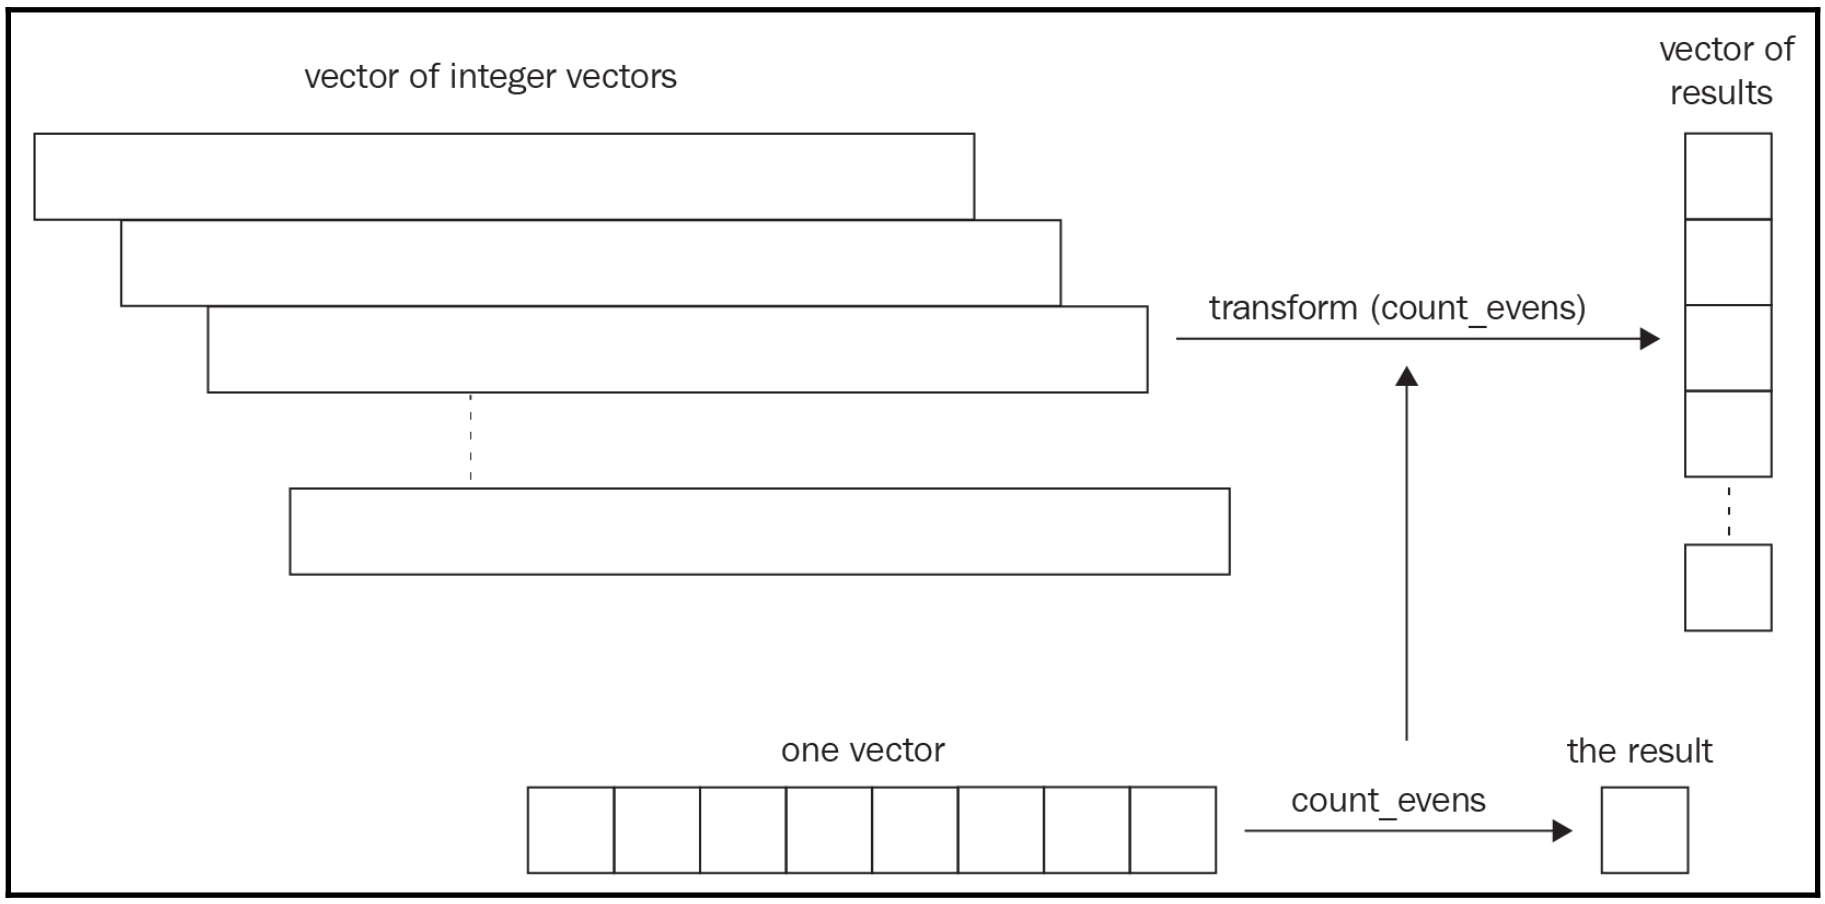
\includegraphics[width=0.6\textwidth]{content/Section-2/Chapter-7/3}
\end{center}

函数式编程的核心是,将较大的问题分解为较小的独立任务。每个函数都专门用于完成一个足够简单的任务,而没有意识到原来的问题。然后将函数组合在一起,从原始的初始输入生成一组已处理的结果。 \par
count\underline{ }all\underline{ }evens()函数的最终版本利用了range。让我们来看看range是什么,以及如何使用它。在后面的例子中,我们还会用到它。 \par

\noindent\textbf{}\ \par
\textbf{使用ranges} \ \par
range与views绑定,我们将在本节中对它们进行研究。它们为我们提供了一种组合和处理对象集合的通用方法。我们经常使用迭代器来遍历容器并处理其元素,迭代器允许我们对算法和容器进行解耦。 \par
例如,我们对vector应用了count\underline{ }if(),但是count\underline{ }if()不知道它会应用于哪种容器。看看以下count\underline{ }if()的声明: \par

\begin{lstlisting}[caption={}]
template <typename InputIterator, typename UnaryPredicate>
constexpr typename iterator_traits<InputIterator>::difference_type
count_if(InputIterator first, InputIterator last, UnaryPredicate p);
\end{lstlisting}

除了C++特有的详细声明之外,count\underline{ }if()不接受容器作为参数。相反,它使用迭代器操作——特别是输入迭代器。 \par

\hspace*{\fill} \\ %插入空行

\includegraphics[width=0.05\textwidth]{images/warn}
输入迭代器支持使用++操作符进行迭代,并支持使用*操作符访问每个元素。还可以使用==和!=关系来比较输入迭代器。 \par
\noindent\textbf{}\ \par

算法遍历容器而不知道容器的确切类型。可以对任何有开始和结束的实体使用count\underline{ }if(),如下所示: \par

\begin{lstlisting}[caption={}]
#include <array>
#include <iostream>
#include <algorithm>
int main()
{
	std::array<int, 4> arr{1, 2, 3, 4};
	auto res = std::count_if(arr.cbegin(), arr.cend(),
		[](int x){ return x == 3; });
	std::cout << "There are " << res << " number of elements equal to 3";
}
\end{lstlisting}

通常,我们对一个集合应用一个算法,并将该算法的结果存储为另一个集合,之后我们以同样的方式将该集合应用于更多算法。使用std::transform()将结果放入另一个容器中。例如,下面的代码定义了一个乘积向量: \par

\begin{lstlisting}[caption={}]
// consider the Product is already declared and has a "name", "price", and
"weight"
// also consider the get_products() is defined
// and returns a vector of Product instances
using ProductList = std::vector<std::shared_ptr<Product>>;
ProductList vec{get_products()};
\end{lstlisting}

假设项目是由不同的程序员团队开发的,他们选择保留产品的名称为任意数字,例如:1代表苹果,2代表桃子,以此类推。这意味着vec将包含Product实例,每个实例在其名称字段中都有一个数字字符(而名称的类型是std::string——这就是为什么我们将数字作为字符而不是其整数值)。现在,我们的任务是将产品名称从数字转换为完整字符串(apple、peach等)。我们可以使用std::transform: \par

\begin{lstlisting}[caption={}]
ProductList full_named_products; // type alias has been defined above
using ProductPtr = std::shared_ptr<Product>;
std::transform(vec.cbegin(), vec.cend(),
	std::back_inserter(full_named_products),
	[](ProductPtr p){ /* modify the name and return */ });
\end{lstlisting}

运行上述代码后,full\underline{ }named\underline{ }products将包含具有产品名的Product。为了过滤掉所有的apple并将它们复制到apple向量中,我们需要使用std::copy\underline{ }if: \par

\begin{lstlisting}[caption={}]
ProductList apples;
std::copy_if(full_named_products.cbegin(), full_named_products.cend(),
	std::back_inserter(apples),
	[](ProductPtr p){ return p->name() == "apple"; });
\end{lstlisting}

代码示例的最大缺点是在引入range之前,缺乏良好的组合。range为我们提供了一种处理容器元素和组合算法的优雅方式。 \par
简单地说,range是一个可遍历的实体,一个range有一个begin()和一个end(),这与目前为止使用的容器非常相似。这些条件下,每个STL容器都可以视为一个range。STL算法重新定义为接受范围作为直接参数,它们允许将一个结果从一个算法直接传递给另一个算法,而不是将中间结果存储在局部变量中。例如,可以在前面在begin()和end()中使用的std::transform,如果使用range,则具有以下形式(以下代码是伪代码)。通过使用range,可以按照以下方式重写前面的例子: \par

\begin{lstlisting}[caption={}]
ProductList apples = filter(
	transform(vec, [](ProductPtr p){/* normalize the name */}),
	[](ProductPtr p){return p->name() == "apple";}
);
\end{lstlisting}

不要忘记包含<ranges>头文件。transform将返回一个包含名称的Product指针的range,也就是将数值替换为字符串值。然后,filter函数将获取结果并返回名称为apple的产品range。 \par

\hspace*{\fill} \\ %插入空行

\includegraphics[width=0.05\textwidth]{images/warn}
注意,我们通过省略简化了这些代码示例
在filter和transform函数前面的std::ranges::views。相应地,使用它们作为std::ranges::views::filter和std::ranges::views::transform。 \par
\noindent\textbf{}\ \par

最后,我们在本章开头的示例中使用了重载操作符|,它允许我们在一起调用管道范围。这样,我们可以组合算法来产生最终结果,如下所示: \par

\begin{lstlisting}[caption={}]
ProductList apples = vec | transform([](ProductPtr p){/* normalize the name
	*/})
| filter([](ProductPtr p){return p->name() ==
	"apple";});
\end{lstlisting}

我们使用管道代替嵌套的函数调用。这一开始可能会令人困惑,因为我们使用|操作符作为位或。当你看到它被应用到一个集合时,它指的是管道范围。 \par

\hspace*{\fill} \\ %插入空行

\includegraphics[width=0.05\textwidth]{images/tip}
|操作符的灵感来自于Unix shell管道操作符。在Unix中,我们可以通过管道将多个进程的结果连接在一起,例如:\texttt{ls -l | grep cpp | less}将在ls命令的结果中找到cpp,并使用less程序一次显示一个屏幕的最终结果。 \par
\noindent\textbf{}\ \par

range是集合之上的抽象,这并不意味着它是一个集合。这就是为什么前面的例子没有任何开销——它只是在一个函数之间传递一个range,这个range只是提供一个集合的开始和结束。此外,还允许我们访问底层的集合元素。下面的图表说明了这个想法: \par

\begin{center}
	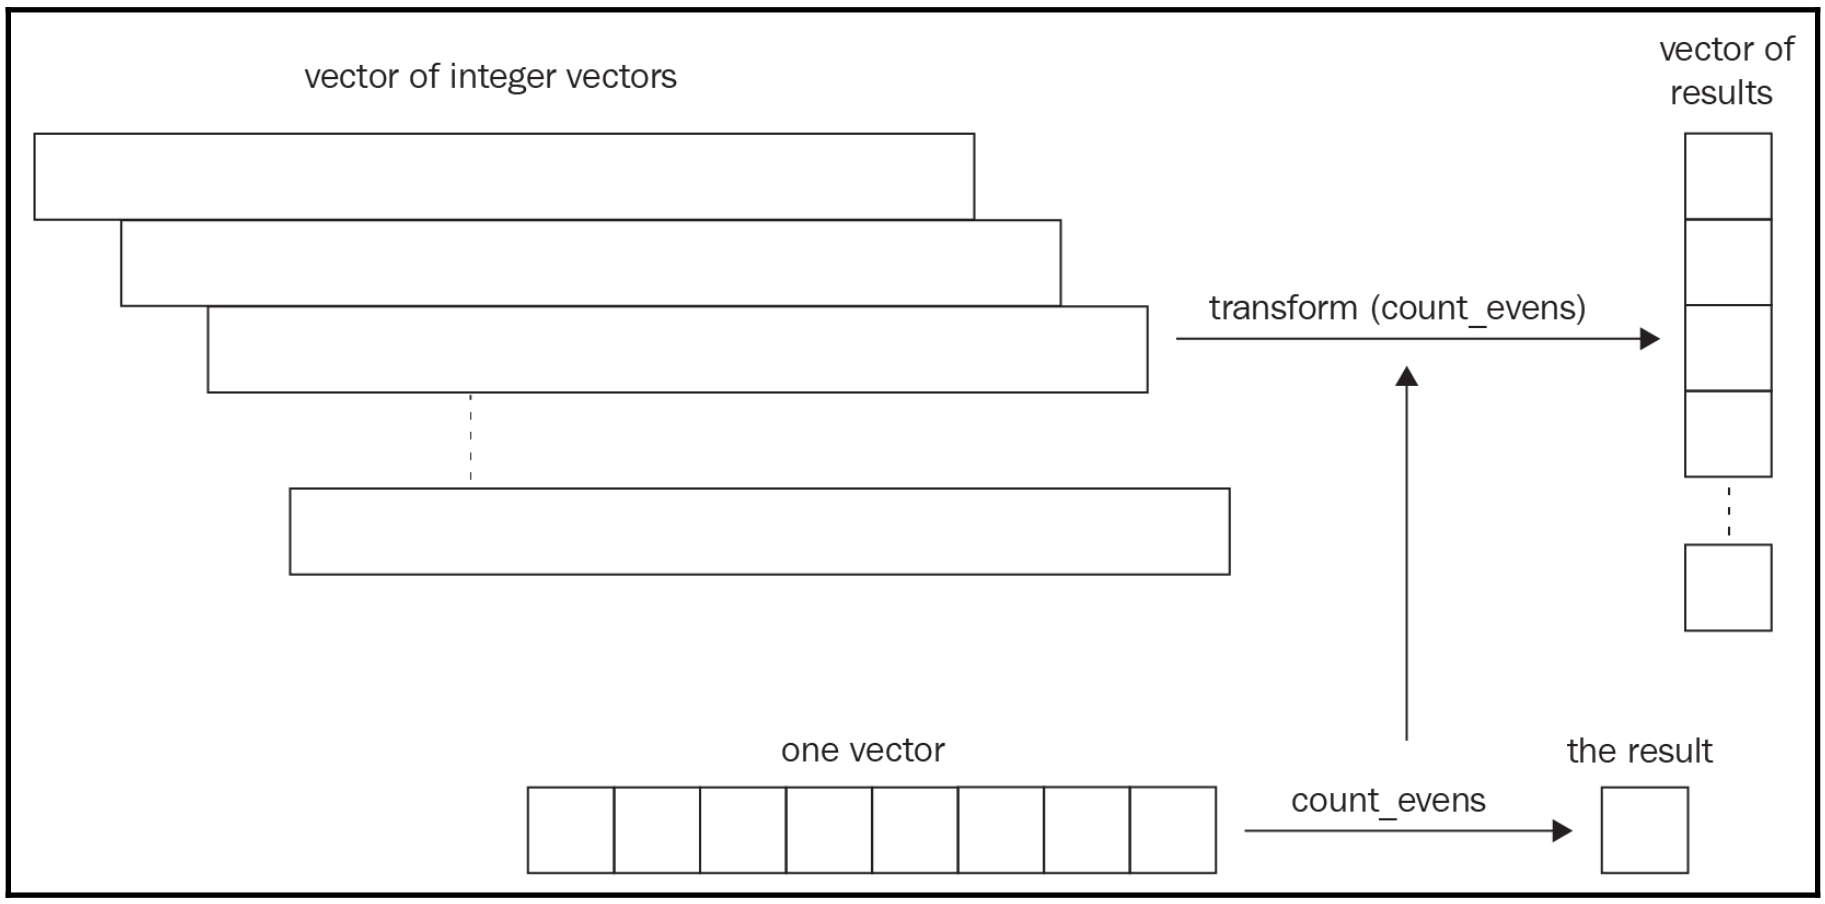
\includegraphics[width=0.6\textwidth]{content/Section-2/Chapter-7/3}
\end{center}

该函数(transform或filter)返回一个范围结构,而不是一个集合。range的begin()迭代器将指向源集合中满足谓词的元素。range的迭代器是一个代理对象:它与常规迭代器的不同之处在于,指向一个满足给定谓词的元素。我们有时将它们称为智能迭代器,因为每次向前移动它(例如,通过递增),都会找到集合中满足谓词的下一个元素。更有趣的是,迭代器的“智能”取决于我们应用于集合的函数类型。例如,filter()函数返回一个范围,该range的自增操作符具有智能迭代器。这主要是因为过滤器的结果可能比原始集合包含更少的元素。另一方面,Transform并不返回元素数量较少的结果——它只是转换元素。这意味着transform返回的range对于自增/自减操作具有相同的功能,但元素访问将有所不同。对于每次访问,range的智能迭代器将从原始集合返回转换后的元素。换句话说,只是为迭代器实现了*操作符,参考下面的代码片段: \par

\begin{lstlisting}[caption={}]
auto operator*()
{
	return predicate(*current_position);
}
\end{lstlisting}

这样,我们就创建了集合的新视图,同样适用于filter和其他函数。更有趣的是,区间视图利用了惰性求值。对于我们前面的示例,即使我们有两个range转换,结果也是通过在一次传递中求值产生的。\par
在transform和filter的示例中,每个函数都定义了一个视图,但不修改或求值。当我们将结果赋值给结果集合时,通过访问每个元素来从视图构造vector。这个vector才是求值的地方。 \par
就是这么简单——range为我们提供了带有惰性求值的函数组合。现在,我们简要地介绍了函数式编程中使用的工具集。接下来,让我们来看看这个范例的优点。 \par

\noindent\textbf{}\ \par
\textbf{为什么使用函数式编程?} \ \par
首先,函数式编程简化了代码。与命令式对应的代码相比,该代码要短得多。它提供了简单但极富表现力的工具。代码越少,bug就越少。 \par
函数不会改变任何东西,这使得并行化更加容易。这是并发程序的主要关注点之一,因为并发任务需要在它们之间共享可变数据。大多数情况下,必须使用互斥对象等显式地同步线程。函数式编程将我们从显式的同步中解放出来,我们可以在多个线程上运行代码而无需进行调整。第8章中,我们将详细讨论数据竞争。 \par
函数式编程认为所有的功能都是纯粹的,是不会改变程序状态的函数。它们只是接受输入,以用户定义的方式对其进行转换,然后提供输出。纯函数对于相同的输入生成相同的结果,而不受调用次数的影响。当我们谈到函数式编程时,在默认情况下,我们应该考虑所有纯函数。 \par
下面的函数接受double作为输入,并返回square: \par

\begin{lstlisting}[caption={}]
double square(double num) { return num * num; }
\end{lstlisting}

只编写纯函数可能会让人感觉,像是故意让程序运行得更慢。 \par

\hspace*{\fill} \\ %插入空行

\includegraphics[width=0.05\textwidth]{images/tip}
有些编译器,如GCC,提供帮助编译器优化代码的属性。例如,[[gnu::pure]]属性告诉编译器这个函数可以被认为是一个纯函数。这将使编译器确信函数不访问任何全局变量,并且函数的结果完全依赖于它的输入。 \par
\noindent\textbf{}\ \par

许多情况下,常规函数可以带来更快的解决方案。然而,为了适应这种模式,应该强迫自己从功能的角度思考。下面的程序声明了一个vector,并计算其元素的平方根: \par

\begin{lstlisting}[caption={}]
void calc_square_roots(std::vector<double>& vec)
{
	for (auto& elem : vec) {
		elem = std::sqrt(elem);
	}
}
int main()
{
	std::vector<double> vec{1.1, 2.2, 4.3, 5.6, 2.4};
	calc_square_roots(vec);
}
\end{lstlisting}

这里,我们通过引用传递向量。如果我们在函数中改变它,我们就改变了原始集合。这显然不是一个纯函数因为它改变了输入向量。而函数式编程将在新的vector中返回计算后的值,而不影响输入: \par

\begin{lstlisting}[caption={}]
std::vector<double> pure_calc_square_roots(const std::vector<double>& vec)
{
	std::vector<double> new_vector;
	for (const auto& elem : vec) {
		new_vector.push_back(std::sqrt(elem));
	}
	return new_vector;
}
\end{lstlisting}

功能性思维的一个更好的例子是,解决一个较小的问题并将其应用到集合中。本例中,较小的问题是计算单个数字的平方根,这个数字已经实现为std::sqrt。将它应用到集合是通过std::ranges::views::transform完成的,如下所示: \par

\begin{lstlisting}[caption={}]
#include <ranges>
#include <vector>

int main()
{
	std::vector<double> vec{1.1, 2.2, 4.3, 5.6, 2.4};
	auto result = vec | std::ranges::views::transform(std::sqrt);
}
\end{lstlisting}

我们使用range,可以避免存储中间对象。前面的例子中,我们直接对向量应用了transform。transform返回一个view,但不是由源向量的已转换元素组成的完整集合,而是在构造结果向量时生成元素的实际转换副本。另外,注意std::sqrt是一个纯函数。 \par
我们在本章开头解决的例子,为函数式编程提供了必要的视角。为了更好地理解这个范式,我们应该熟悉它的原理。下一节中,我们将深入研究函数式编程的原理,以便更好地了解如何,以及何时使用范例。 \par

\noindent\textbf{}\ \par
\textbf{函数式编程原理} \ \par
尽管函数范式已经很老了(它诞生于20世纪50年代),但它并没有席卷编程界。目前占主导地位的大多数范式包括命令式语言和面向对象语言。正如我们在本书和其他许多书中多次提到的,C++是一种多范式语言。这就是学习C++的好处:我们可以调整它以适应几乎所有的环境。掌握范式并不是一件容易的事。必须感受它并应用它,直到你最终开始从范例的角度思考。之后,将在几秒钟内看到常规任务的解决方案。 \par
如果还记得第一次学习面向对象编程是什么时候,那么可能还记得在能够释放OOP的真正潜力之前,那些有些难懂的原则,函数式编程也是如此。本节中,我们将讨论函数式编程的基本概念,这些概念将成为进一步开发的基础。可以应用(或者已经这样做了)其中的一些概念,而无需实际使用功能范例。然而,请努力理解并应用下面的每一条原则。 \par

\noindent\textbf{}\ \par
\textbf{纯函数} \ \par

\noindent\textbf{}\ \par
\textbf{高阶函数} \ \par

\noindent\textbf{}\ \par
\textbf{折叠表达式} \ \par

\noindent\textbf{}\ \par
\textbf{深入地研究递归} \ \par

\noindent\textbf{}\ \par
\textbf{头递归} \ \par

\noindent\textbf{}\ \par
\textbf{尾递归} \ \par

\noindent\textbf{}\ \par
\textbf{C++中(函数式)的元编程} \ \par

\noindent\textbf{}\ \par
\textbf{总结} \ \par

\noindent\textbf{}\ \par
\textbf{问题} \ \par
\begin{enumerate}
	\item 列出range的优点。
	\item 已知哪些函数是纯函数?
	\item 从函数式编程的角度来看,纯虚函数和纯函数有什么区别?
	\item 什么是折叠表达式?
	\item 尾递归比头递归有什么好处?
\end{enumerate}

\noindent\textbf{}\ \par
\textbf{扩展阅读} \ \par
有关本章内容的更多信息,请查看以下链接: \par

\begin{itemize}
	\item Learning C++ Functional Programming by Wisnu Anggoro:  https:/​/​www.packtpub.​com/​application-​development/​learning-​c-​functional-​programming
	\item Functional Programming in C++: How to Improve Your C++ Programs Using Functional Techniques by Ivan Cukic:  https:/​/​www.​amazon.​com/​Functional-Programming-​programs-​functional-​techniques/​dp/​1617293814/​
\end{itemize}

\newpage







